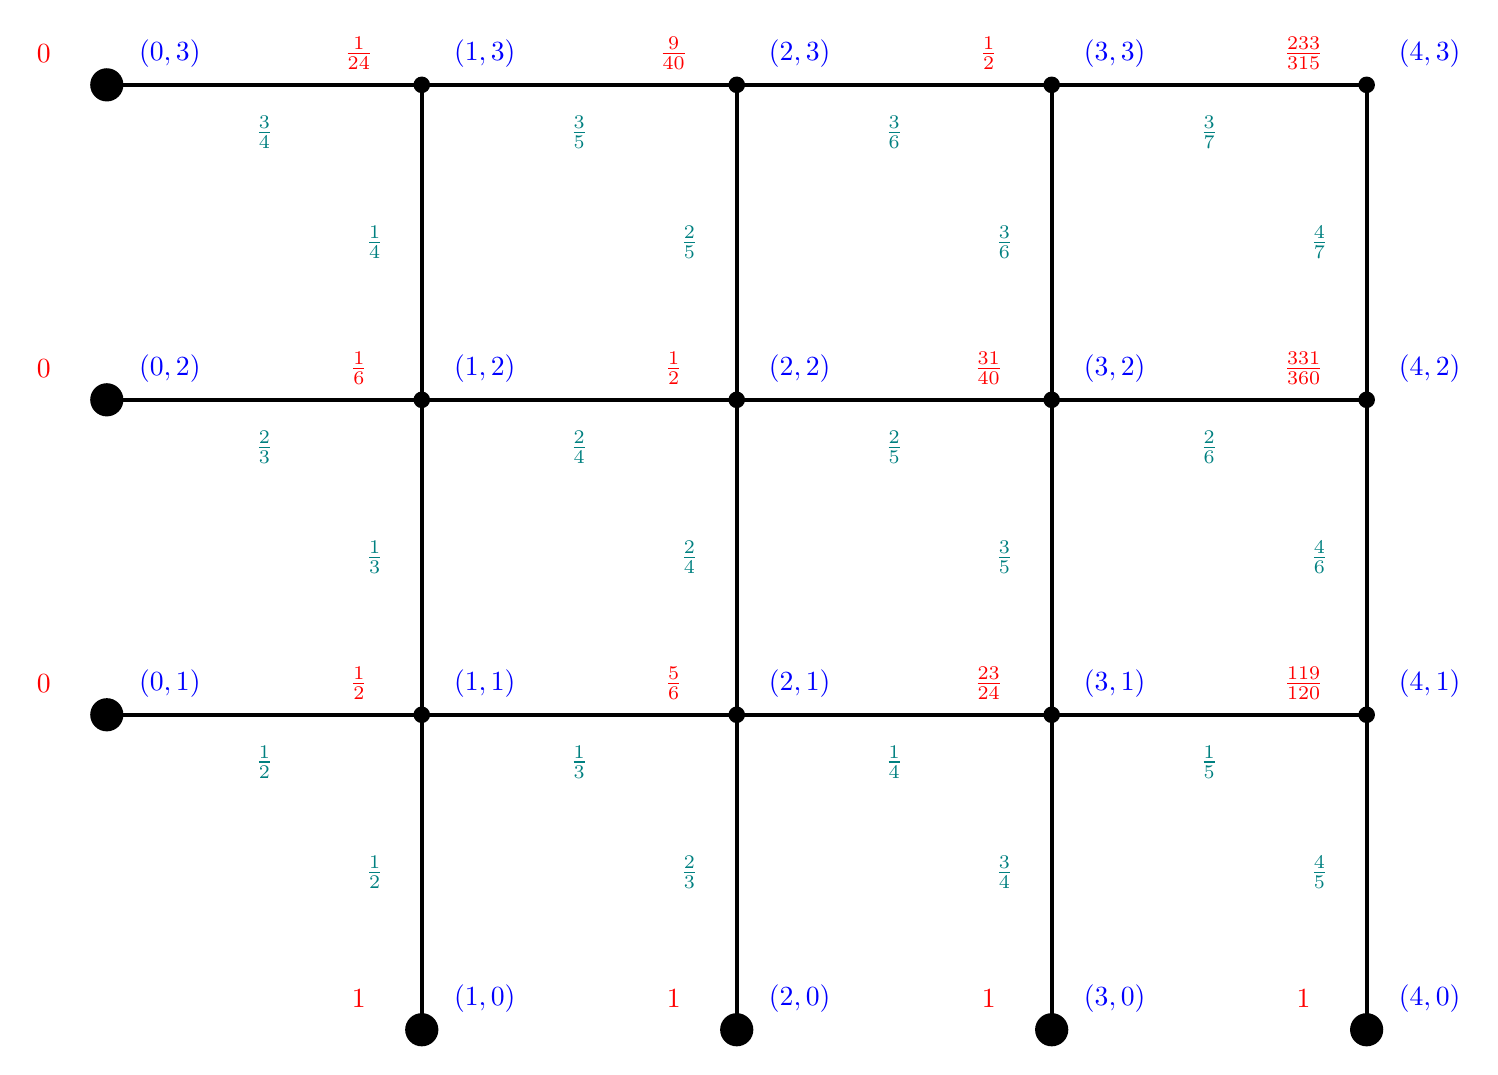
\begin{tikzpicture}[line cap=round,line join=round,x=4cm,y=4cm]


\fill (1,0) circle[radius=6pt];
\fill (2,0) circle[radius=6pt];
\fill (3,0) circle[radius=6pt];
\fill (4,0) circle[radius=6pt];
\fill (0,1) circle[radius=6pt];
\fill (1,1) circle[radius=3pt];
\fill (2,1) circle[radius=3pt];
\fill (3,1) circle[radius=3pt];
\fill (4,1) circle[radius=3pt];
\fill (0,2) circle[radius=6pt];
\fill (1,2) circle[radius=3pt];
\fill (2,2) circle[radius=3pt];
\fill (3,2) circle[radius=3pt];
\fill (4,2) circle[radius=3pt];
\fill (0,3) circle[radius=6pt];
\fill (1,3) circle[radius=3pt];
\fill (2,3) circle[radius=3pt];
\fill (3,3) circle[radius=3pt];
\fill (4,3) circle[radius=3pt];

\draw[line width=0.5mm] (1,1) -- (0,1) node[sloped, pos=0.5, allow upside down]{\arrowIn};
\draw[line width=0.5mm] (2,1) -- (1,1) node[sloped, pos=0.5, allow upside down]{\arrowIn};
\draw[line width=0.5mm] (3,1) -- (2,1) node[sloped, pos=0.5, allow upside down]{\arrowIn};
\draw[line width=0.5mm] (4,1) -- (3,1) node[sloped, pos=0.5, allow upside down]{\arrowIn};
\draw[line width=0.5mm] (1,2) -- (0,2) node[sloped, pos=0.5, allow upside down]{\arrowIn};
\draw[line width=0.5mm] (2,2) -- (1,2) node[sloped, pos=0.5, allow upside down]{\arrowIn};
\draw[line width=0.5mm] (3,2) -- (2,2) node[sloped, pos=0.5, allow upside down]{\arrowIn};
\draw[line width=0.5mm] (4,2) -- (3,2) node[sloped, pos=0.5, allow upside down]{\arrowIn};
\draw[line width=0.5mm] (1,3) -- (0,3) node[sloped, pos=0.5, allow upside down]{\arrowIn};
\draw[line width=0.5mm] (2,3) -- (1,3) node[sloped, pos=0.5, allow upside down]{\arrowIn};
\draw[line width=0.5mm] (3,3) -- (2,3) node[sloped, pos=0.5, allow upside down]{\arrowIn};
\draw[line width=0.5mm] (4,3) -- (3,3) node[sloped, pos=0.5, allow upside down]{\arrowIn};

\draw[line width=0.5mm] (1,1) -- (1,0) node[sloped, pos=0.5, allow upside down]{\arrowIn};
\draw[line width=0.5mm] (1,2) -- (1,1) node[sloped, pos=0.5, allow upside down]{\arrowIn};
\draw[line width=0.5mm] (1,3) -- (1,2) node[sloped, pos=0.5, allow upside down]{\arrowIn};
\draw[line width=0.5mm] (2,1) -- (2,0) node[sloped, pos=0.5, allow upside down]{\arrowIn};
\draw[line width=0.5mm] (2,2) -- (2,1) node[sloped, pos=0.5, allow upside down]{\arrowIn};
\draw[line width=0.5mm] (2,3) -- (2,2) node[sloped, pos=0.5, allow upside down]{\arrowIn};
\draw[line width=0.5mm] (3,1) -- (3,0) node[sloped, pos=0.5, allow upside down]{\arrowIn};
\draw[line width=0.5mm] (3,2) -- (3,1) node[sloped, pos=0.5, allow upside down]{\arrowIn};
\draw[line width=0.5mm] (3,3) -- (3,2) node[sloped, pos=0.5, allow upside down]{\arrowIn};
\draw[line width=0.5mm] (4,1) -- (4,0) node[sloped, pos=0.5, allow upside down]{\arrowIn};
\draw[line width=0.5mm] (4,2) -- (4,1) node[sloped, pos=0.5, allow upside down]{\arrowIn};
\draw[line width=0.5mm] (4,3) -- (4,2) node[sloped, pos=0.5, allow upside down]{\arrowIn};



\node[text=blue] at (1.2, 0.1)  {$(1,0)$};
\node[text=blue] at (2.2, 0.1)  {$(2,0)$};
\node[text=blue] at (3.2, 0.1)  {$(3,0)$};
\node[text=blue] at (4.2, 0.1)  {$(4,0)$};
\node[text=blue] at (0.2, 1.1)  {$(0,1)$};
\node[text=blue] at (1.2, 1.1)  {$(1,1)$};
\node[text=blue] at (2.2, 1.1)  {$(2,1)$};
\node[text=blue] at (3.2, 1.1)  {$(3,1)$};
\node[text=blue] at (4.2, 1.1)  {$(4,1)$};
\node[text=blue] at (0.2, 2.1)  {$(0,2)$};
\node[text=blue] at (1.2, 2.1)  {$(1,2)$};
\node[text=blue] at (2.2, 2.1)  {$(2,2)$};
\node[text=blue] at (3.2, 2.1)  {$(3,2)$};
\node[text=blue] at (4.2, 2.1)  {$(4,2)$};
\node[text=blue] at (0.2, 3.1)  {$(0,3)$};
\node[text=blue] at (1.2, 3.1)  {$(1,3)$};
\node[text=blue] at (2.2, 3.1)  {$(2,3)$};
\node[text=blue] at (3.2, 3.1)  {$(3,3)$};
\node[text=blue] at (4.2, 3.1)  {$(4,3)$};

%  probs for horizontal lines:
\node[text=teal] at (0.5, 0.85)  {$\frac{1}{2}$};
\node[text=teal] at (1.5, 0.85)  {$\frac{1}{3}$};
\node[text=teal] at (2.5, 0.85)  {$\frac{1}{4}$};
\node[text=teal] at (3.5, 0.85)  {$\frac{1}{5}$};
\node[text=teal] at (0.5, 1.85)  {$\frac{2}{3}$};
\node[text=teal] at (1.5, 1.85)  {$\frac{2}{4}$};
\node[text=teal] at (2.5, 1.85)  {$\frac{2}{5}$};
\node[text=teal] at (3.5, 1.85)  {$\frac{2}{6}$};
\node[text=teal] at (0.5, 2.85)  {$\frac{3}{4}$};
\node[text=teal] at (1.5, 2.85)  {$\frac{3}{5}$};
\node[text=teal] at (2.5, 2.85)  {$\frac{3}{6}$};
\node[text=teal] at (3.5, 2.85)  {$\frac{3}{7}$};


%  probs for vertical lines:
\node[text=teal] at (0.85, 0.5)  {$\frac{1}{2}$};
\node[text=teal] at (1.85, 0.5)  {$\frac{2}{3}$};
\node[text=teal] at (2.85, 0.5)  {$\frac{3}{4}$};
\node[text=teal] at (3.85, 0.5)  {$\frac{4}{5}$};
\node[text=teal] at (0.85, 1.5)  {$\frac{1}{3}$};
\node[text=teal] at (1.85, 1.5)  {$\frac{2}{4}$};
\node[text=teal] at (2.85, 1.5)  {$\frac{3}{5}$};
\node[text=teal] at (3.85, 1.5)  {$\frac{4}{6}$};
\node[text=teal] at (0.85, 2.5)  {$\frac{1}{4}$};
\node[text=teal] at (1.85, 2.5)  {$\frac{2}{5}$};
\node[text=teal] at (2.85, 2.5)  {$\frac{3}{6}$};
\node[text=teal] at (3.85, 2.5)  {$\frac{4}{7}$};


\node[text=red] at ( 0.8, 0.1)  {$1$};
\node[text=red] at ( 1.8, 0.1)  {$1$};
\node[text=red] at ( 2.8, 0.1)  {$1$};
\node[text=red] at ( 3.8, 0.1)  {$1$};
\node[text=red] at (-0.2, 1.1)  {$0$};
\node[text=red] at ( 0.8, 1.1)  {$\frac{1}{2}$};
\node[text=red] at ( 1.8, 1.1)  {$\frac{5}{6}$};
\node[text=red] at ( 2.8, 1.1)  {$\frac{23}{24}$};
\node[text=red] at ( 3.8, 1.1)  {$\frac{119}{120}$};
\node[text=red] at (-0.2, 2.1)  {$0$};
\node[text=red] at ( 0.8, 2.1)  {$\frac{1}{6}$};
\node[text=red] at ( 1.8, 2.1)  {$\frac{1}{2}$};
\node[text=red] at ( 2.8, 2.1)  {$\frac{31}{40}$};
\node[text=red] at ( 3.8, 2.1)  {$\frac{331}{360}$};
\node[text=red] at (-0.2, 3.1)  {$0$};
\node[text=red] at ( 0.8, 3.1)  {$\frac{1}{24}$};
\node[text=red] at ( 1.8, 3.1)  {$\frac{9}{40}$};
\node[text=red] at ( 2.8, 3.1)  {$\frac{1}{2}$};
\node[text=red] at ( 3.8, 3.1)  {$\frac{233}{315}$};
\end{tikzpicture}
